\graphicspath{{chapters/notes/07/images/}}

\chapter{Tumor evolution studies: SNVs-based methods}

\section{Introduction}

    \subsection{Copy-number neutral tumours}
    There is a large number of tumours where copy-number aberrations are minimal.
    These tumours are said to have quiet genomes and make about $1$ to $3\%$ of all primary tumours, like the one in figure \ref{fig:quiet}.
    Consequently, it is difficult to use copy number based approaches for these kind of tumours as they display very few copy number changes.
    These tumours are typically correlated to a better prognosis both in overall survival and in progression-free interval, but relapses are still present so the assessment of these tumours is important.

    \begin{figure}[H]
    \centering
        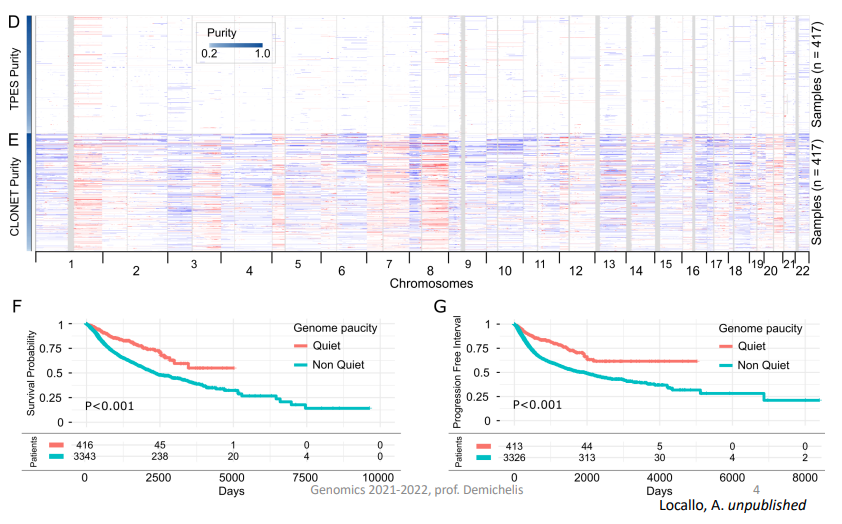
\includegraphics[width=0.7\linewidth]{quiet_genome.png}
        \caption{Data on quiet genomes.}
        \label{fig:quiet}
    \end{figure}

    \subsection{Different methods for tumour assessment}
    Multiple Tumor Purity Assessment assays have been proposed, based on:
    \begin{multicols}{3}
        \begin{itemize}
            \item RNA.
            \item DNA methylation.
            \item SNVs.
        \end{itemize}
    \end{multicols}

    This chapter focuses on methods exploiting SNVs.

    \subsection{Rationale of SNV based methods}
    Figure \ref{fig:snv-intro-cluster} depicts the call for $2$ SNV respectively in $2$ genomic loci $P_1$ and $P_2$.
    Let $A$ be the reference allele and $B$ the alternative one associated with a somatic point mutation.
    Three populations of cells are considered:

    \begin{multicols}{3}
        \begin{itemize}
            \item Normal cells show a genotype of $AA$ for $P_1$ and $AA$ for $P_2$.
            \item Clonal cells show a genotype of $AB$ for $P_1$ and $AA$ for $P_2$.
            \item Subclonal cells show a genotype of $AB$ for $P_1$ and $AB$ for $P_2$.
        \end{itemize}
    \end{multicols}

    It can be seen how the distribution of allelic fraction of the clonal population (B-E) is symmetric, with the main peak around $0.5$.
    A mixed population of clonal tumour and normal healthy cells show a peak shifted toward $0$ (C-F), as healthy cells don't carry the mutation.
    The distance from $0.5$ is proportional to the fraction of normal cells.
    A subclonal population (D-F) is identified thanks to a second peak of allelic fraction closer to $0$.

    \begin{figure}[H]
        \centering
        \begin{tabular}{cc}
          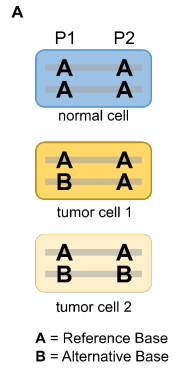
\includegraphics[width=0.2\textwidth]{SNVs.png} &   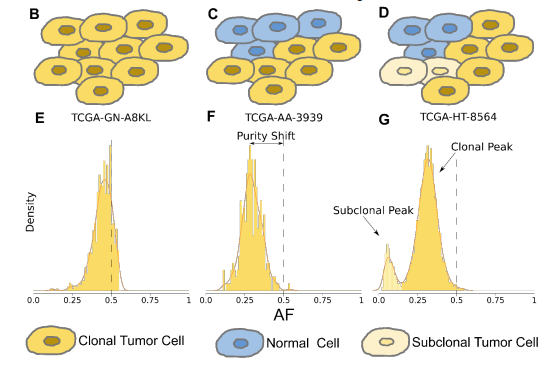
\includegraphics[width=0.5\textwidth]{peaks.png} \\
        (a)  & (b)  \\[6pt]
        \end{tabular}
        \caption{Allelic fraction change for SNVs in a clonal, subclonal and admixed tumour cell population.}
        \label{fig:snv-intro-cluster}
    \end{figure}

    \subsection{Advantages and limitations of SNVs based methods}
    Advantages and limitations of SNVs based methods are described in table \ref{tab:snv-pro-cons}.

    \begin{table}[H]
        \centering
        \begin{tabular}{|c|c|}
            \hline
            Advantages & Limitations\\
            \hline
            \makecell{Best suited for copy number\\ neutral tumour genomes.} & \multirow{2}{*}{\makecell{Needs a reasonable number of putative clonal\\somatic heterozygous SNVs per sample.}}\\
            \cline{1-1}
            \makecell{Applicable to a range\\of NGS techniques.} & \\
            \hline
            \makecell{Fast and low demanding\\of computational resources.} & \multirow{2}{*}{\makecell{Sensible to subclonal cell populations which\\could influence clonal peak detection.}}\\
            \cline{1-1}
            \makecell{TPES is available as\\an R package on CRAN.} &\\
            \hline
        \end{tabular}
        \caption{Advantages and limitations of SNVs based methods}
        \label{tab:snv-pro-cons}
    \end{table}

    \subsection{Reference mapping bias}
    When performing an SNV based itest it is important to consider the Reference Mapping Bias.
    A polymorphic locus carrying a non-reference base is less likely to be mapped during the alignment process.
    With a perfect SNV that is clonal, monoallelic and in highly pure tumour, the allelic fraction will not be at $0.5$ because the aligner considers the variation as an error and sometimes discards the read containing it loosing some signal with a bias for the alternative base.

\section{TPES - tumour purity estimation from SNVs}

    \subsection{Introduction}
    TPES (tumour purity estimation from SNVs) is a tool able to assess the purity of a tumour sample basing its process on the detection of SNVs.
    The process that the tool employs is depicted in figure \ref{fig:tpes}

    \begin{figure}[H]
    \centering
        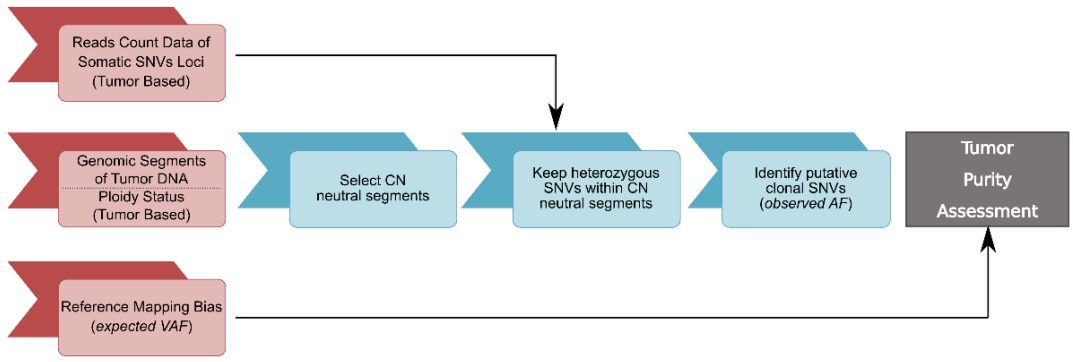
\includegraphics[width=0.7\linewidth]{tpes.png}
        \caption{Workflow of the TPES tool}
        \label{fig:tpes}
    \end{figure}

    \subsection{SNV identification}
    TPES pays great attention in which SNV chooses to perform purity assessment.
    The choice is done in different steps considering different property of each SNV.
    In particular it selects SNVs according to:

    \begin{multicols}{2}
        \begin{itemize}
            \item SNVs in copy number neutral segments.
            \item Allelic fraction threshold.
            \item Identification of putative clonal SNVs.
        \end{itemize}
    \end{multicols}

        \subsubsection{Selection of copy-number neutral segments}
        TPES selects for point mutations that are flat in terms of copy-number.
        These are perfect for flat genomes and easier to deal with.
        This is the first filter implemented by this tool: a threshold is set on the $\log_2 R$ to filter the segments in which SNVs are searched.

        \subsubsection{Allelic fraction}
        Considering all of the somatic point mutations of whole genome, a major peak is expected around $0.5$.
        This is called expected VAF.
        Other peaks can be originated from things that escaped the previous filter or from monoallelic mutations with copy-neutral loss of heterozygosity.
        In this case the allelic fraction results doubled.
        TPES poses another threshold on the allelic fraction to filter out all the SNVs deriving from these segment: the $\max AF$ allowed is of $0.55$.

        \subsubsection{Identification of putative clonal SNVs}
        TPES ranks all the remaining SNV according to their allelic fraction: the peak closer to $0.5$ is the most useful to determine tumour purity.
        This is because the others are related to subclonal events.

    \subsection{Purity estimation}
    With enough point mutations and after peaks identification the purity is computed as:

    $$1-purity = admixture = 1-\frac{observed\ VAF}{expected\ VAF}$$

    \subsection{Minimal number of SNV for tumour identification}
    The number of SNVs changes for each tumour type, so not all tumour types guarantee enough SNVs.
    The minimum number of SNVs needed to obtain reliable results can be assessed with a comparative analysis.
    Spearman's correlations between the results of two different purity caller algorithms (TPES and CLONET) using decreasing number of SNVs are computed.
    SNVs are subsampled as many times as possible to increase the confidence on the results.
    At each iteration as many samples as possible are used, but the number of samples available decreases as the number of SNVs increases.
    These statistical test determined $10$ as the minimum number of SNVs needed to infer tumour purity, as reported in figure \ref{fig:comp}.
    With this number, tumour content was detected in $80\%$ of the samples by combining TPES and CLONET, which is copy-number based.
    The $20\%$ could be tumour-free or samples non detected.
    Since both SNVs and CN based methods failed, the tumour content of the remaining $20\%$ could be possibly detected with methylation analysis.

    \begin{figure}[H]
    \centering
        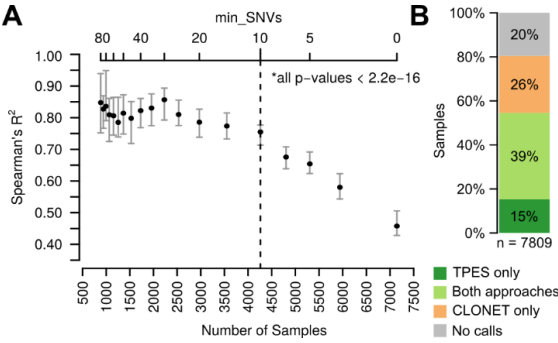
\includegraphics[width=0.7\linewidth]{comparative.png}
        \caption{\textbf{A}) Correlation between TPES and CLONET with decreasing number of SNVs. \textbf{B)} Percentages of samples where tumour purity was assessed considering $10$ SNVs.}
        \label{fig:comp}
    \end{figure}

    \subsection{Comparison with other tumour callers}
    TPES was compared to other tumour purity caller with a range of different methodologies: good correlation between the results was found, in particular with copy number based algorithms.
    This shows that genomics is more reproducible in general to assess purity, while methods relying for example on image analysis give different results.
    The best solution to assess tumour purity is to couple a copy number-based and a SNV-based approach: some samples are only detected by one of the two so a combination gives the best results globally.
